\documentclass[12pt,a4paper]{article}
% 如果需要中文支持,推荐使用xeCJK + 字体设置
\usepackage{xeCJK}
\setCJKmainfont{SimSun}  % 示例:宋体,可根据系统字体情况更换
\usepackage{amsmath}      % 数学公式(如有需要)
\usepackage{graphicx}     % 插图
\usepackage{geometry}     % 调整页边距
\usepackage{fancyhdr}     % 自定义页眉页脚
\usepackage{indentfirst}  % 中文首行缩进
\usepackage{calc}         % 允许做长度运算(测量文字宽度等)
\usepackage{titlesec}
\usepackage{booktabs} % 解决 \midrule 和 \bottomrule 报错
\usepackage{enumitem} % 支持自定义列表格式
\usepackage{float}    % 支持强制浮动位置

% 设置 \section 级标题为:加粗、大字号(如 \Large)
\titleformat{\section}
	{\bfseries\large}    % 标题自身的格式
	{\thesection}        % 标题编号的显示方式
	{1em}                % 编号与标题文字之间的间距
	{}                   % 在标题文字前后可插入额外代码,此处为空
	
% 设置 \subsection 级标题为:加粗、中等字号(如 \normalsize)
\titleformat{\subsection}
	{\bfseries\normalsize}
	{\thesubsection}
	{1em}
{}

% 页面设置(可根据需要微调)
\geometry{
	left=2cm,
	right=2cm,
	top=1cm,
	bottom=1.5cm
}

% 不需要过大的行距,使用较接近单倍行距的设置
\renewcommand{\baselinestretch}{1}

% 仅在页脚居中显示页码,页眉保持为空
\pagestyle{fancy}
\fancyhf{}  % 清空默认的页眉页脚
\fancyfoot[C]{\thepage}
\renewcommand{\headrulewidth}{0pt}
\renewcommand{\footrulewidth}{0pt}

% 首行缩进2字符(中文习惯)
\setlength{\parindent}{0pt}
\setlength{\leftskip}{2em}

\begin{document}
	%-------------------------------------------------------
	% 1 并排两个minipage:左标题、右校徽
	%   - 0.65\textwidth + 0.35\textwidth = \textwidth
	%   - 如果校徽过大或过小,可改宽度,如 0.25\textwidth、0.3\textwidth 等
	%   - 如果想让标题更大,可将 \Huge 改成 \huge 或 \LARGE
	%-------------------------------------------------------
	\noindent
	\hspace{-2em}
	\begin{minipage}[c]{0.65\textwidth}
		\raggedright
		{\fontsize{40pt}{60pt}\selectfont 物理实验报告}
	\end{minipage}
	\begin{minipage}[c]{0.35\textwidth}
		\raggedleft
		% 强制把校徽拉大到 0.35\textwidth 宽度 (高度自动匹配)
		% 若想指定高度,可用 "height=3cm" 等. 二选一即可.
		
\includegraphics[width=\linewidth, trim={20cm 20cm 20cm 20cm}, clip]{university_logo.png}
	\end{minipage}

	\vspace{-1em}
	

	%下方画两条分割线,并在两线之间写学号、姓名、日期、时间
	
	\hrule
	\vspace{0.4em}
	\noindent
	\begin{tabular}{l l l l}
    学号:\underline{114514} & 姓名:\underline{SUSTecher} &
    日期:\underline{2025/03/04} & 时间:\underline{周二下午}
	\end{tabular}
	\vspace{-0em}
	\par
	\hrule

	
	\section{实验名称:时间测量中随机误差的分布规律}
	
	\section{实验目的}
	认识多次重复等精度测量过程中随机误差的离散性和分布规律,学习直接测量量的不确定度计算和表示方法。

	\section{实验原理}
	本实验使用秒表重复测量电子节拍器的周期T0,测量结果计为T1,T2,\dots,Tn。
	如果测量次数足够多,那么测量结果处于T附近的概率密度趋近于正态分布,如下公式
	$$p(T)=\frac{1}{\sigma\sqrt{2\pi}}exp[-\frac{(T-\bar{T})^2}{2\sigma^2}]$$
	其中,$\bar{T}=\frac{1}{n}\sum_{j=1}^{n}T_j$ 表示周期测量值的平均值,$\sigma=\sqrt{\sum_{j=1}^{n}(T_j-\bar{T})^2/(n-1)}$ 表示周期测量值的标准差。
	正态分布理论表明,测量结果处于 $\sigma$, $2\sigma$, $3\sigma$ \text{ 置信区间的 P 值不同,即}

	\begin{table}[h]
		\centering % 表格居中
		\renewcommand{\arraystretch}{2.0} % 调整行距,1.3 为示例,可根据需要调整
		\begin{tabular}{|c|c|c|c|}
			\hline
			置信区间 & $[\overline{T}-\sigma,\overline{T}+\sigma]$ & $[\overline{T}-2\sigma,\overline{T}+2\sigma]$ & $[\overline{T}-3\sigma,\overline{T}+3\sigma]$ \\ \hline
			计算公式 & $\int_{\bar{T}-\sigma}^{\bar{T}+\sigma} p(T) dT$ & $\int_{\bar{T}-2\sigma}^{\bar{T}+2\sigma} p(T) dT $ & $\int_{\bar{T}-3\sigma}^{\bar{T}+3\sigma} p(T) dT $ \\ \hline
			理论值 & 0.6827 & 0.9545 & 0.9973 \\ \hline
		\end{tabular}
		\caption{测正态分布理论置信区间值} % 添加表格标题
		\label{tab:confidence_intervals} % 添加引用标签
	\end{table}
	
	基于标准差,可以计算周期测量的A类标准不确定度
	$$u_A=\frac{\sigma}{\sqrt{n}}$$
	
	本次实验中,周期测量的 B 类标准不确定度主要来源于实验者的估计误差(反应时间:开、停共计两次秒表反应时间:2 x 0.1s=0.2s)$\Delta_{\text{估}}$ 和秒表的仪器误差 $\Delta_{\text{仪}}$(约为0.01s)
	\[u_B=\sqrt{\Delta_{\text{估}}^2+\Delta_{\text{仪}}^2}/C\]
	其中,C 为置信系数。两类不确定度的合成和扩展公式为:\[u_P=\sqrt{(t_Pu_A)^2+(k_Pu_B)^2}\]
	其中,$k_{P}$和$t_{P}$分别为置信因子和$t$因子。 
	\\最后,节拍器周期测量结果表示为\[T=\bar{T}\pm u_P,P=0.95\]
	
	\section{实验仪器}
	电子节拍器,秒表

	\section{实验内容}
	1.用秒表测量电子节拍器周期,测量$n$组数据,$n=200$。
	\\2. 计算测量结果的平均值$\bar{T}$和标准差$\sigma$。
	\\3.根据测量结果的离散程度和极限差$R=T_{max}-T_{min}$,合理设置小区间步长$\Delta T$和个数$K$。
	\\4. 统计区间$[T_i-\Delta T/2,T_i+\Delta T/2]$内的频率$n_i$(数据点个数)、概率$P_i$($n_i/n$)和概率密度$p_i$($P_i/\Delta T$),并绘制$p_i$随区间中值$T_i$变化的直方图。
	\\5. 计算正态分布函数$p(T)=\frac1{\sigma\sqrt{2\pi}}exp[-\frac{(T-\bar{T})^2}{2\sigma^2}]$在各中值$T_i$位置的函数值。
	\\6. 在 $p_i \sim T_i$ 直方图上添加 $p(T_i) \sim T_i$ 散点图,检验测量结果是否符合正态分布。
	\\7. 分别统计测量结果出现在置信区间$[\bar{T}-\sigma,\bar{T}+\sigma]$,$[\bar{T}-2\sigma,\bar{T}+2\sigma]$ 和$\lceil\bar{T}-3\sigma,\bar{T}+3\sigma\rceil$内的概率$P$,并与理论值比较。
	\\8. 计算测量结果的$A$类标准不确定度和$B$类标准不确定度,并写出置信概率为$P=0.95$时的测量结果完整表达式。
	
	\section{数据记录}
	用秒表测量电子节拍器周期,记录200组测量数据

	\section{数据处理}
	1. 使用 Excel 统计处理测量数据,得出平均值 $\overline{T}=3.0521s$,标准差 $\sigma=0.075452338$(未处理数据见附表)。

	\begin{table}[h]
    	\centering
    	\renewcommand{\arraystretch}{1.3} % 调整行距
    	\begin{tabular}{l c}
        	\toprule
        	\textbf{基础统计数据} & \\
        	\midrule
        	平均值   & 3.0521 \\
        	标准误差 & 0.005335286 \\
        	中位数   & 3.06 \\
        	众数     & 3.03 \\
        	标准差   & 0.075452338 \\
        	方差     & 0.005693055 \\
        	峰度     & 0.312070258 \\
        	偏度     & 0.238444988 \\
        	极差     & 0.46 \\
        	最小值   & 2.88 \\
        	最大值   & 3.34 \\
        	求和     & 610.42 \\
        	观测数   & 200 \\
        	\bottomrule
    	\end{tabular}
    	\caption{测量数据的基础统计分析}
    	\label{tab:stats}
	\end{table}
	
	2.根据实验数据的离散程度和最值$T_{\max}=3.34,T_{\min}=2.88$,极差$R=T_{\max}-T_{\min}=0.46$,设小区间步长$\Delta T=0.05$,个数K=12
		\begin{figure}[H]
		\centering
		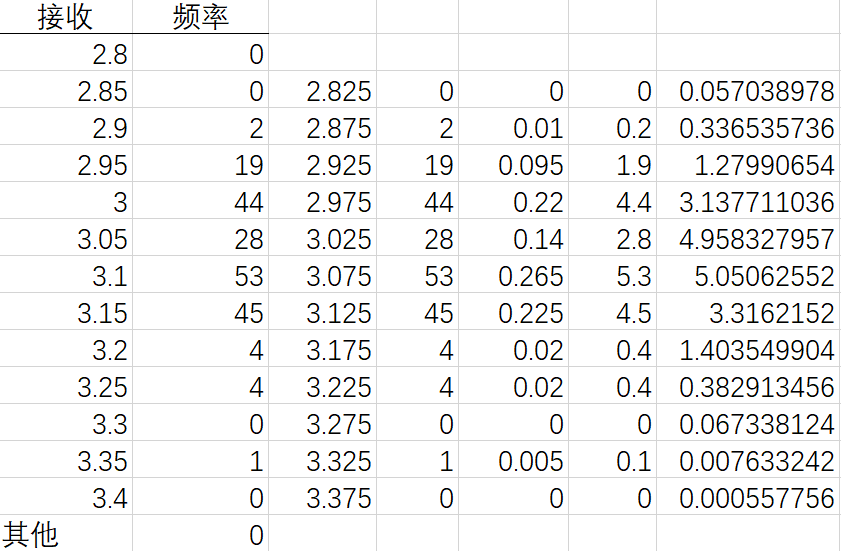
\includegraphics[width=0.4\textwidth]{图一.png}
		\caption{数据计算}
		\label{fig:chart1}
	\end{figure}


	3.根据统计数据计算正态分布函数$f(T)=\frac{1}{\sqrt{2\pi}\sigma}e^{-\frac{(T-\bar{T})^2}{2\sigma^2}}$,绘制相应直方图和散点图
	\begin{figure}[H]
		\centering
		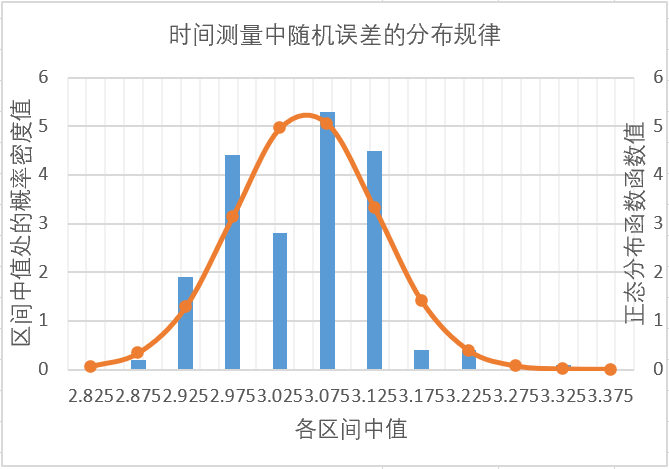
\includegraphics[width=0.6\textwidth]{图二.png}
		\caption{时间测量中随机误差的分布规律}
		\label{fig:chart1}
	\end{figure}
	
	4.分别统计测量结果出现在置信区间内的概率,并与理论值比较,发现接近。表明测量结果基本符合正态分布。
	\[[\overline{T}-\sigma,\overline{T}+\sigma]\text{区间}: [2.9767, 3.1275], \text{个数:}136, \text{概率:}0.6800\]
	\[[\overline{T}-2\sigma,\overline{T}+2\sigma]\text{区间}: [2.9013, 3.2029], \text{个数:}192, \text{概率:}0.9600\]
	\[[\overline{T}-3\sigma,\overline{T}+3\sigma]\text{区间}: [2.8258, 3.2784], \text{个数:}199, \text{概率:}0.9950\]
	\begin{table}[h]
		\centering % 表格居中
		\renewcommand{\arraystretch}{1.3} % 调整行距,1.3 为示例,可根据需要调整
		\begin{tabular}{|c|c|c|c|}
			\hline
			置信区间 & $[\overline{T}-\sigma,\overline{T}+\sigma]$ & $[\overline{T}-2\sigma,\overline{T}+2\sigma]$ & $[\overline{T}-3\sigma,\overline{T}+3\sigma]$ \\ \hline
			概率 & 0.6800 & 0.9600 & 0.9950 \\ \hline
			理论值 & 0.6827 & 0.9545 & 0.9973 \\ \hline
		\end{tabular}
		\caption{测量结果的置信区间分析} % 添加表格标题
		\label{tab:confidence_intervals} % 添加引用标签
	\end{table}
	
	5.不确定度计算
	A类不确定度:
		$$u_{A}=\frac{\sigma}{\sqrt{n}}=\frac{0.0754523377794347}{\sqrt{200}}=0.005335s$$
	
	B类不确定度:
		\[u_B=\sqrt{\Delta_{\text{估}}^2+\Delta_{\text{仪}}^2}/C=\frac{\sqrt{(0.2)^{2}+(0.01)^{2}}}{3}=0.0668s\]
		$\text{估计误差}\,\Delta_{\text{估}}\text{源于人开、停秒表反应时间:}0.2\,\text{s}$
		$\quad \Delta_{\text{仪}} = 0.01\,\text{s}\text{(使用秒表)}$

	不确定度的合成:$(P=0.95)$
		$$t_{0.95}=1.96 \quad k_{0.45}=1.96$$
		$$u_{p}=\sqrt{(t_{0.95}u_{A})^{2}+(k_{0.95}u_{B})^{2}}=\sqrt{(1.96\times0.005335)^{2}+(1.96\times0.0668)^{2}}=0.1313s$$

	6.测量结果完整表达式
	$$T=(3.0521\pm0.1313)s\quad(P=0.95)$$

	\section{问题思考}
	\begin{enumerate}[leftmargin=2em, label=\arabic*.]
		\item 若测量结果偏离正态分布,可能的主要原因包括:
		\begin{enumerate}[label=(\alph*)]
			\item \textbf{非随机干扰因素:} 测量过程中可能存在环境波动、实验者操作习惯等非随机因素未完全随机化,从而破坏了独立同分布的前提,导致数据偏离正态分布。
			\item \textbf{数据异常或离群值:} 操作失误或记录错误产生的极端值会拉伸分布尾部,使整体分布偏离理想的钟形曲线。
			\item \textbf{样本量不足:} 当重复测量次数较少时,随机误差未能充分体现正态分布特性,从而导致观测数据与理论分布存在差异。
			\item \textbf{仪器精度与数据离散化:} 仪器精度有限时,测量结果可能被取整,造成数据间隔较大,从而影响连续性,导致分布偏离正态分布。
		\end{enumerate}
	
		\item 在不考虑系统误差的前提下,多次等精度测量的随机误差分布通常具有以下特征:
		\begin{enumerate}[label=(\alph*)]
			\item \textbf{特征性:} 误差分布通常符合数学统计规律,其统计特征可以通过参数(如均值、标准差等)来描述。
			\item \textbf{单峰性:} 误差分布通常呈现单峰形态,即在均值附近出现最高峰,并向两侧对称下降。
			\item \textbf{有界性:} 误差值不会无限增大或减小,通常在一定范围内变化,极端误差出现的概率较小。
			\item \textbf{抵偿性:} 由于误差是随机分布的,在多次测量中,正误差与负误差相互抵消,使得总体测量值接近真实值。
		\end{enumerate}
	\end{enumerate}
	
	\section{实验结论}
	本实验使用秒表重复测量200次电子节拍器的周期T,并利用统计学方法计算得到实验记录电子节拍器周期满足正态分布曲线,为:
	$$T=(3.0521\pm0.1313)s\quad(P=0.95)$$
	通过本实验,揭示了多次重复等精度测量过程中存在随机误差的离散性和分布规律,但有概率接近正态分布曲线,且正态分布曲线具有统计学规律。

	

\end{document}
